\chapter{Results and Discussion}

\section{Identification of Significant Features}

This project employs unsupervised learning, specifically a K-means clustering algorithm, to identify the most relevant features for describing pain. This is done by generating clusters, where K is the number defined by the user for the quantity of centroids \cite{Ikotun2023}. The clustering technique partitions data according to specific distance metrics, and `cityblock' was chosen because of the way centroids are computed, that is, as the component-wise median of points in each cluster. Besides this, this metric measures the sum of absolute differences between data point coordinates, and assigns points to clusters based on this distance. This clustering algorithm was applied to every possible pair of features, with the number of centroids set to $K=2$, using data from the second baseline and from the pain stimulation phase of the fifteen participants. It's important to mention that this analysis was firstly done with the first baseline but, comparing both options, the results were better using the second one, which may stem from the influence of the emotional stimuli in the pain felt by the participants.

The result of clustering applied to two features -- the medians of the entropy of db4 detail (x-axis) and of db4 approximation (y-axis) -- is displayed in Figure \ref{fig:cluster} (right). In it, two clusters can be seen, as well as X's in the position of the clusters' centroids.
For comparison, scattering graphics were plotted for each two features, as can be seen in Figure \ref{fig:cluster} (left). The incorrect matches made by the clustering algorithm are circled in black.

\begin{figure}[h!]
    \centering
    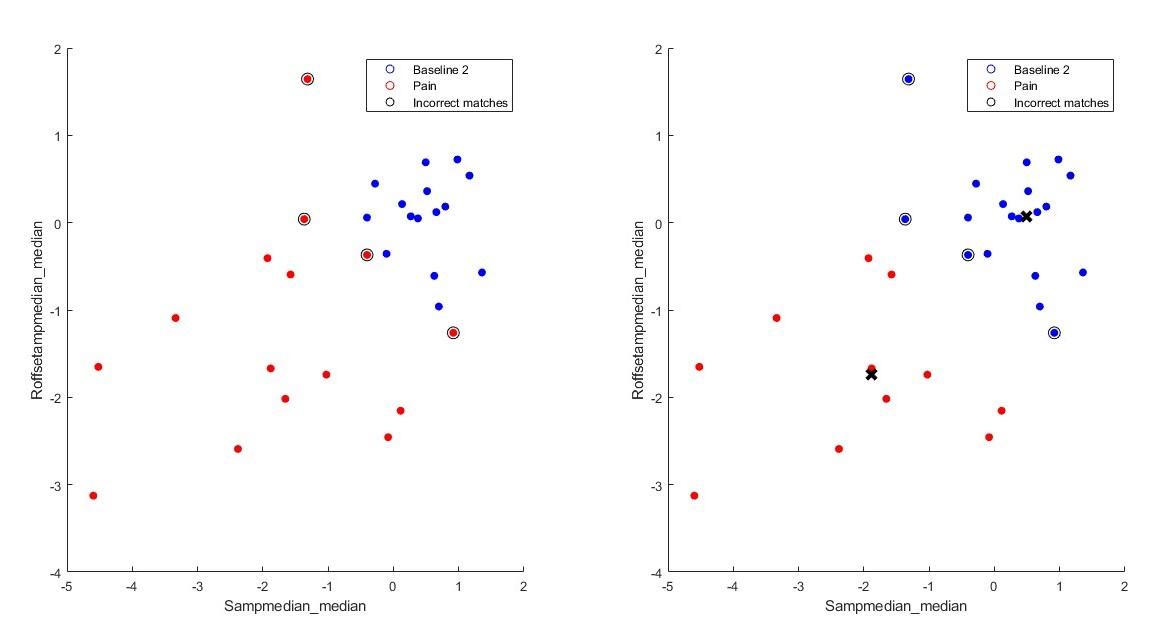
\includegraphics[width=1.0\textwidth]{cluster.jpg}
    \caption{Scattering plot with data from baseline 2 and pain (left), and with the result of K-means clustering (right), when comparing the medians of the entropy of db4 detail and db4 approximation.}
    \label{fig:cluster}
\end{figure}

Only the pairs of features where clustering was done with over 80\% accuracy were considered valid. A network map illustrating these results was plotted in Figure \ref{fig:map80}. In this map, each circle corresponds to a feature, while the lines connecting them showcase the combinations that met the accuracy threshold. Additionally, the size of the circles is proportional to how many times that specific feature, paired with another, contributed to successful clustering. These results suggest that these five features, Roffsetampmedian\_median, Sampmedian\_median, Entropydb4Approx\_median, Entropydb4Detail\_median, and Entropydb9Detail\_median, when paired with each other, are the most effective in distinguishing pain from no pain. 



\begin{figure}[h!]
    \centering
    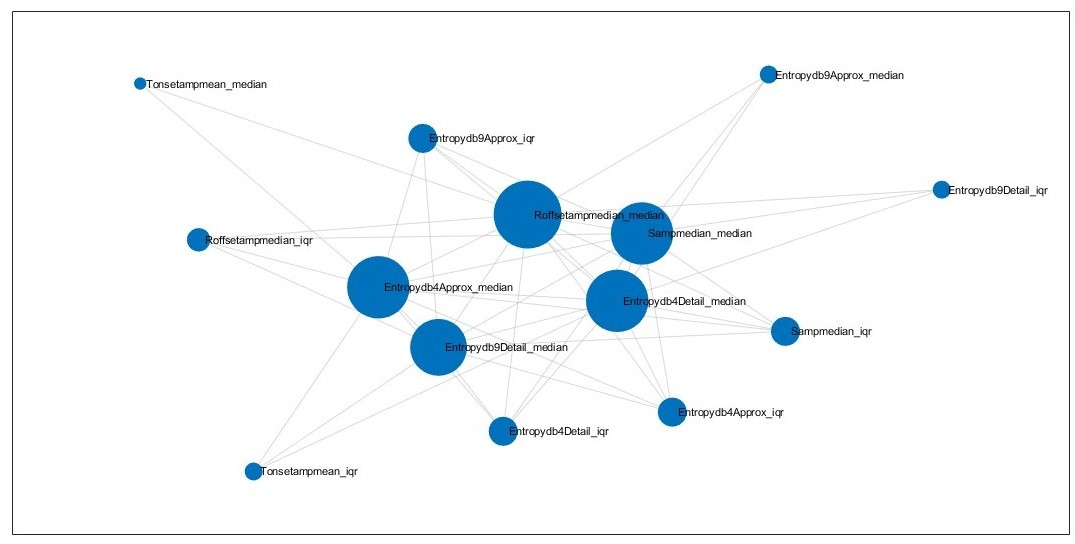
\includegraphics[width=1.0\textwidth]{map80.jpg}
    \caption{Network diagram of the pairs of features with more than 80\% accuracy of clustering.}
    \label{fig:map80}
\end{figure}

To determine whether these features can distinguish pain from the lack of it in spite of the situation, a multiple comparison test was applied to both the baselines and to the pain phase. To do this, a one-way \ac{anova} was applied to the three groups. This test evaluates whether there are statistically significant differences between the means of each group. Afterwards, Tukey-Kramer method, also known as the \ac{hsd} method, was performed as a post-hoc test.
The result of this test is portrayed in Figure \ref{fig:five_images}.




\begin{figure}[htbp]
    \centering
    % First row of 2 images
    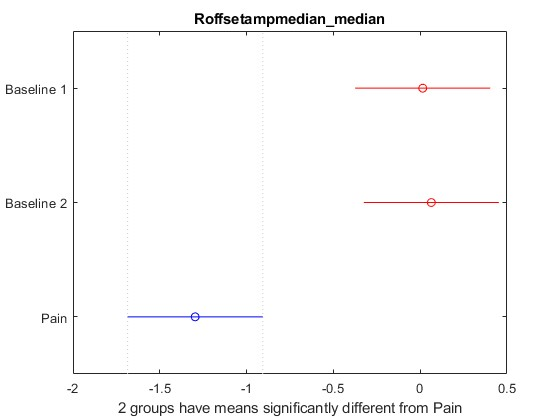
\includegraphics[width=0.48\linewidth]{multcompareR.jpg}
    \hfill
    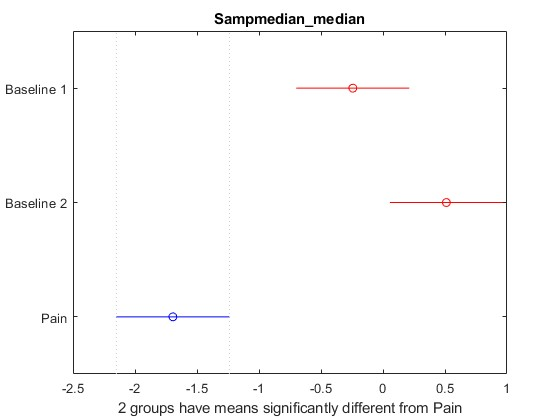
\includegraphics[width=0.48\linewidth]{multcompareS.jpg}
    \vspace{0.5em}  % space between rows
    % Second row of 2 images
    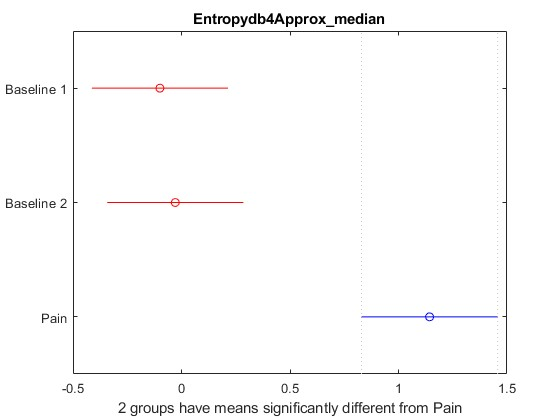
\includegraphics[width=0.48\linewidth]{multcompare4approx.jpg}
    \hfill
    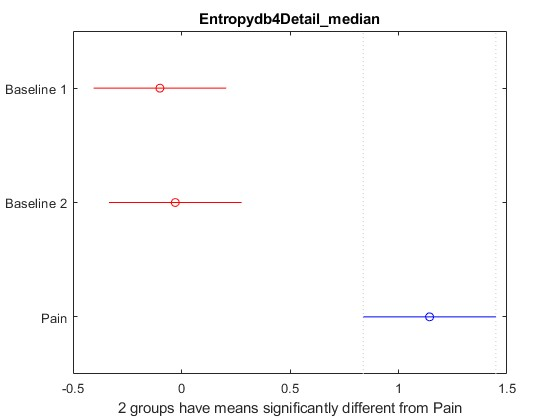
\includegraphics[width=0.48\linewidth]{multcompare4detail.jpg}
    \vspace{0.5em}  % space between rows
    % Third row with 1 centered image
    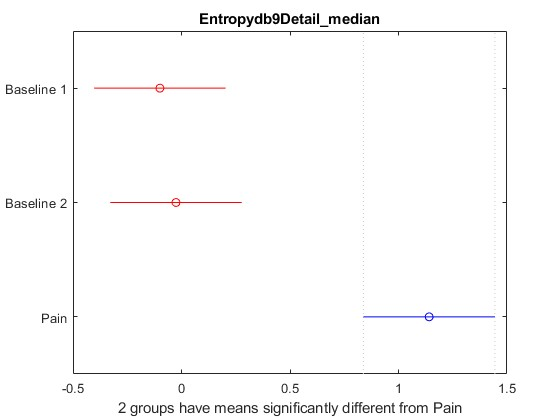
\includegraphics[width=0.48\linewidth]{multcompare9detail.jpg}
    \caption{Multiple comparison test applied to both the baselines and to the pain phase, for each of the selected features.}
    \label{fig:five_images}
\end{figure}





